%{\tiny }%# -*- coding:utf-8 -*-
\documentclass[10pt,aspectratio=169,mathserif]{beamer}
%设置为 Beamer 文档类型,设置字体为 10pt,长宽比为16:9,数学字体为 serif 风格

%%%%-----导入宏包-----%%%%
\usepackage{zju}			%导入 zju 模板宏包
\usepackage{ctex}			%导入 ctex 宏包,添加中文支持
\usepackage{amsmath,amsfonts,amssymb,bm}   %导入数学公式所需宏包
\usepackage{color}			 %字体颜色支持
\usepackage{graphicx,hyperref,url}
\usepackage{metalogo}	% 非必须
%% 上文引用的包可按实际情况自行增删
%%%%%%%%%%%%%%%%%%
\usepackage{fontspec}
\usepackage{xeCJK}
% \setCJKmainfont{Source Han Sans SC}



\beamertemplateballitem		%设置 Beamer 主题

%%%%------------------------%%%%%
\catcode`\。=\active         %或者=13
\newcommand{。}{.}
%将正文中的“。”号转换为“.”。中文标点国家规范建议科技文献中的句号用圆点替代
%%%%%%%%%%%%%%%%%%%%%

%%%%----首页信息设置----%%%%
\title[ 分形函数水平集的基本性质]{分形函数水平集的基本性质}
\subtitle{——从Takagi函数到广义的Takagi函数}
%%%%----标题设置


\author[Kangjie Lou]{
  楼康杰 \\\medskip
  指导老师:阮火军
  }
%%%%----个人信息设置

\institute[IOPP]{
  数学科学学院 \\
  浙江大学}
%%%%----机构信息

\date[May 16 2025]{
  2025年5月16日}
%%%%----日期信息

\begin{document}

	\begin{frame}
		\titlepage
	\end{frame}				%生成标题页

	\section{目录}
		\begin{frame}
			\frametitle{目录}
			\tableofcontents
		\end{frame}				%生成提纲页

	\section{研究背景及意义}
		\begin{frame}
			\frametitle{研究背景及意义}
 分形几何学起源于19世纪末和20世纪初,研究具有自相似性和复杂结构的几何对象。经典的分形函数如Weierstrass函数、Takagi函数等,在数学上具有独特性质。水平集是函数取相同值的点集合,其研究在分形几何学中重要,分形函数的水平集近年来有重要成果。
本研究聚焦广义Takagi函数水平集,拓展于汉研究成果,揭示其部分维数特征。

		\end{frame}

	\section{研究过程及方法}
		\begin{frame}
			\frametitle{Takagi函数}
			\begin{definition}[Takagi函数]
				$T(x):\mathbb{R}\rightarrow\mathbb{R}$周期为$1$,在区间$[0,1]$上定义如下:
				$$
					T(x)=\begin{cases}
					x~~~~~~,x\in[0,\frac{1}{2}],\\
					1-x~,x\in[\frac{1}{2},1].
				\end{cases}
				$$
				当$0<a<1,b>1$时,定义以下函数$T_{a,b}(x)$为Takagi函数,
				$$
					T_{a,b}(x)=\sum_{n=0}^\infty a^nT(b^nx),
				$$

			\end{definition}

		\end{frame}

		\begin{frame}
			\frametitle{几个重要的定义}
			\begin{definition}[$x$以$b$为基数的展开形式]
				定义$x\in[0,1]$以$b$为基数的展开形式为$x=\sum_{n=1}^{\infty}x_ib^{-i}$,其中$x_i\in\{0,1,\cdots,b-1\}$,并记$x=0.x_1x_2\cdots x_n\cdots.$
			\end{definition}

			\begin{definition}[Littlewood多项式]
				定义系数取值仅为$1,-1$的$k$阶多项式为Littlewood多项式,即
				$$
					\sum_{n=0}^k\epsilon_nx^n=0.
				$$
				其中$\epsilon_n\in\{1,-1\}$。
			\end{definition}
		\end{frame}

		\begin{frame}
			\frametitle{几个重要的定义}
			\begin{definition}[水平集]
				$f:[0,1]\rightarrow\mathbb{R}$,$f(x)=y$的水平集定义为
				$L(y)=\{x\in[0,1]:f(x)=y\}\times\{y\}.$
			\end{definition}

			\begin{definition}[Hausdorff维数]
				$F$的Hausdorff维数定义为
				$$
				\mathrm{\dim_H}F=\inf\Big\{s:\forall\delta>0,\exists\{U_i\}_{i=1}^\infty,\mbox{使得}\bigcup_{i=1}^\infty U_i\supset F,\mbox{且}\sum_{i=1}^\infty (\mathrm{diam}~U_i)^s<\delta\Big\}.
				$$
			\end{definition}
			\begin{definition}[Assouad维数]
				$F$的Assouad维数定义为
				$$
				\mathrm{\dim_A}F=\inf\Big\{s:(\exists C>0)(\forall R>0)\big(\forall r\in(0,R)\big)(\forall x\in F),N_r\big(B(x,R)\cap F\big)\le C\Big(\frac{R}{r}\Big)^s\Big\}.
				$$
			\end{definition}
		\end{frame}

		\begin{frame}
		\frametitle{几个重要的定义}
					\begin{definition}
			对区间$I$,我们用$|I|$表示区间的长度。
		\end{definition}
		\begin{definition}
			给定区间族$\mathbb{I}=\{I_1,I_2,\cdots,I_N\}$,若$\forall i,j,\frac{|I_i|}{|I_j|}\in\mathbb{Q}$,则定义
			$$
			\gcd(\mathbb{I})=\sup\big\{T:\frac{|I_i|}{T}\in\mathbb{Z},i=1,2,\cdots,N\big\}.
			$$
			对区间族$\mathbb{I}$中的区间$I_i$,定义
			$$
			n(I_i)=\frac{|I_i|}{gcd(\mathbb{I})},i=1,2,\cdots,N.
			$$
			显然,对任意的$1\le i\le N,n(I_i)\in\mathbb{Z}$。
			定义$n(\mathbb{I})=\sum_{i=1}^Nn(I_i)$。
		\end{definition}

	\end{frame}

		\begin{frame}
			\frametitle{核心方法}
			于汉在其文章内研究了Takagi函数水平集的一些性质,其文章的核心为,当$ab$为$k-1$阶Littlewood多项式的根,即,
			$$
				\sum_{n=0}^{k-1}\epsilon_n(ab)^n=0,
			$$
			且$2|b$时,则$\exists y\in\mathbb{R}$,使得,
			$$
				\mathrm{\dim_H}L(y)\ge\frac{1}{k}.
			$$
			我将文中的核心方法归纳为以下两个步骤:
			\begin{enumerate}
				\item 将函数部分和与Littlewood多项式相结合。
				\item 通过系数确定来构建$x$的取值区间。
			\end{enumerate}
		\end{frame}

		\begin{frame}
			\frametitle{部分和与Littlewood多项式的结合}
			取$T_{a,b}(x)$的前$k$项部分和,记为$F_1(x)$,
			$$
				F_1(x)=\sum_{n=0}^{k-1}a^nT(b^nx),
			$$
			对上式求导,可得
			$$
				F_1'(x)=\sum_{n=0}^{k-1}(ab)^nT'(b^nx).
			$$
			若能找到一些$x$的值或一些区间,使$T'(b^nx)=\epsilon_n,\epsilon_n\in\{1,-1\}$,则可得$F_1'(x)=0$,从而可得$F'_1(x)$的水平集。
		\end{frame}


		\begin{frame}
			\frametitle{构建$x$的取值区间}
			\begin{figure}
				\caption{T(x)的图像}
				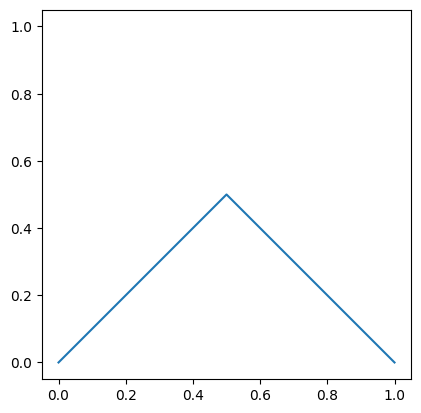
\includegraphics[height=2cm]{"./figures/T.png"}
			\end{figure}
			我们记$\epsilon_n(x)=T'(b^nx)$.通过图像,我们不难得到
			$$
				T'(b^nx)=T'(x_1x_2\cdots x_n.x_{n+1}\cdots x_kx_{k+1}\cdots)=T'(0.x_{n+1}\cdots x_kx_{k+1}\cdots)=\begin{cases}
					1,x_{n+1}\in[0,\frac{b}{2})\\
					-1,x_{n+1}\in[\frac{b}{2},b).
				\end{cases}
			$$
			从而,我们只要选择合适的$x_1,\cdots,x_k$,便可使$F_1'(x)=0$,而这样取$x$得到的是一个连续的区间。
		\end{frame}

		\begin{frame}
			\frametitle{构建$x$的取值区间}
			$$
				F_2(x)=\sum_{n=k}^{2k-1}a^nT(b^nx)=\sum_{n=0}^{k-1}a^n\cdot a^kT(b^n\cdot b^kx)=a^kF_1(b^kx).
			$$
			对上式求导,可得
			$$
				F_2'(x)=(ab)^kF_1'(b^kx).
			$$
			此时采用相同的取值规则,选定合适的$x_{k+1},\cdots,x_{2k}$即可使$F_2'(x)=0$。
			依次类推,我们可以得到$T_{a,b}(x)$的水平集。
		\end{frame}

		\begin{frame}
			\frametitle{从Takagi函数开始的推广思路}

			\begin{figure}[H]
				\caption{$T_2(x)$:改变导数值}
				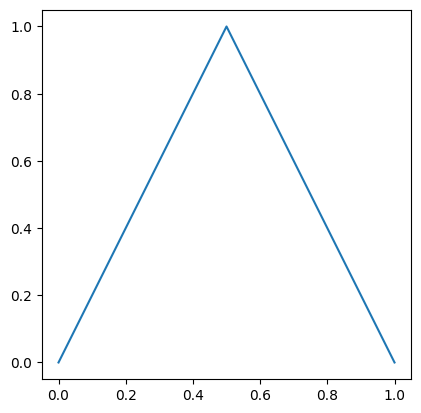
\includegraphics[height=2cm]{"./figures/T2.png"}
			\end{figure}

			这影响了第一步,在对部分和求导时,
			$$
				F_1'(x)=\sum_{n=0}^{k-1}(ab)^nT_2'(b^nx).
			$$
			我们不能让$T_2'(b^nx)=\epsilon_n,\epsilon_n\in\{1,-1\}$,这里应该让$T_2'(b^nx)=2\epsilon_n,$$\epsilon_n\in\{1,-1\}$,此时
			$$
				F_1'(x)=\sum_{n=0}^{k-1}(ab)^nT_2'(b^nx)=\sum_{n=0}^{k-1}2\epsilon_n(ab)^n=2\sum_{n=0}^{k-1}\epsilon_n(ab)^n=0.
			$$

		\end{frame}


		\begin{frame}
			\frametitle{从Takagi函数开始的推广思路}
			以下两种情况影响了第二步,影响了$x_i$的取值区间的数量。
			\begin{columns}
				\column{0.5\textwidth}
				\begin{figure}[H]
					\caption{$T_3(x)$:在中间增加导数为0的区间}
					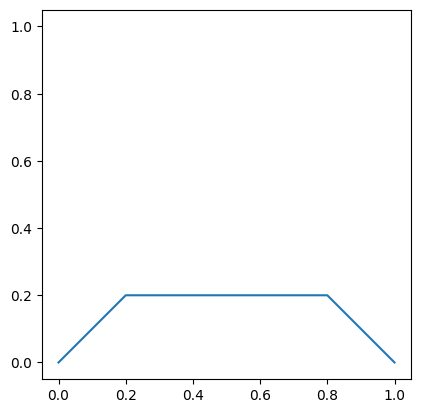
\includegraphics[height=2cm]{"./figures/T3.png"}
				\end{figure}
				$$
					T'(b^nx)=
					\begin{cases}
					1,x_{n+1}\in[0,\frac{b}{5})\\
					0,x_{n+1}\in[\frac{b}{5},\frac{4b}{5})\\
					-1,x_{n+1}\in[\frac{4b}{5},b).
					\end{cases}
				$$
				\column{0.5\textwidth}
				\begin{figure}[H]
					\caption{$T_4(x)$:增加更多区间,但导数仅 为1,0,-1}
					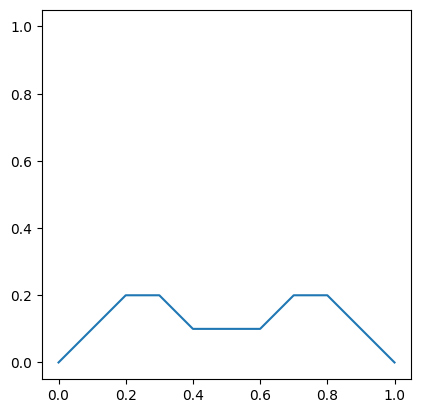
\includegraphics[height=2cm]{"./figures/T4.png"}
				\end{figure}
				$$
					T'(b^nx)=
					\begin{cases}
						1,x_{n+1}\in[0,\frac{b}{5})\cup[\frac{3b}{5},\frac{7b}{10})\\
						0,x_{n+1}\in[\frac{b}{5},\frac{3b}{10})\cup[\frac{2b}{5},\frac{3b}{5})\cup[\frac{7b}{10},\frac{4b}{5})\\
						-1,x_{n+1}\in[\frac{3b}{10},\frac{2b}{5})\cup[\frac{4b}{5},b).
					\end{cases}
				$$
			\end{columns}

		\end{frame}

		\begin{frame}
			\frametitle{从Takagi函数开始的推广思路}

			\begin{figure}[H]
				\caption{任意导数}
				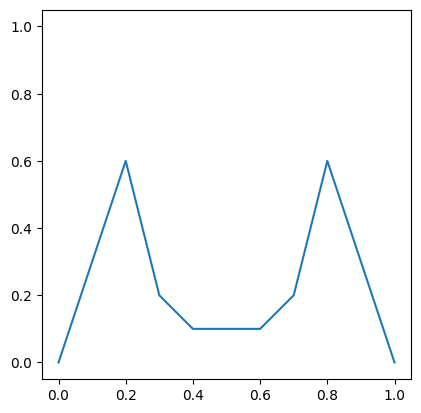
\includegraphics[height=4cm]{"./figures/T5.png"}
			\end{figure}
			这样的函数同时影响了两个步骤,为了不出现部分区间上可以同时取多个值的情况,我们要求由不可导点分割得到的任意两个导数不变的区间长度的比值为有理数。
			这样,我们就将Takagi函数水平集的构推广到了这样一类广义的Takagi函数上,并给出了它的一个水平集的Hausdorff维数的下界。

		\end{frame}


	\section{研究成果}
		\begin{frame}
			\frametitle{取得的结论}

			\begin{theorem}[广义Takagi函数水平集的Hausdorff维数]
				假设$h(x)$为可分割函数,其在$[0,1]$上按$h(x)$的不可导点被分割的区间族为$\mathbb{I}=\{I_1,I_2,\cdots,I_N\}$,其中$I_1,\cdots,I_N$从左到右排列。设$\mathbb{I}$中$h(x)$的导数不为$0$的区间中,区间长度最大的为$I_{J^*}$。
				若广义Takagi函数
				$$
				H_{a,b}(x)=\sum_{n=0}^\infty a^nh(b^nx),
				$$
				满足$0<a<1,b>1$,$ab$为$k-1$阶Littlewood多项式的根,且$n(\mathbb{I})|b$,则存在$y\in\mathbb{R}$,使得
				$$
				\mathrm{dim_H}L(y)\ge\frac{1}{k}\Big(1+\log_b2|I_{J^*}|\Big).
				$$
			\end{theorem}
		\end{frame}

		\begin{frame}
			\frametitle{取得的结论}
			\begin{theorem}[广义Takagi函数的Assouad维数]
				假设$h(x)$为可分割函数,其在$[0,1]$上按$h(x)$的不可导点被分割的区间族为$\mathbb{I}=\{I_1,I_2,\cdots,I_N\}$,其中$I_1,\cdots,I_N$从左到右排列。设$\mathbb{I}$中$h(x)$的导数不为$0$的区间中,区间长度最大的为$I_{J^*}$。
				若广义Takagi函数
				$$
				H_{a,b}(x)=\sum_{n=0}^\infty a^nh(b^nx),
				$$
				满足$0<a<1,b>1,1<ab<2,n(\mathbb{I})|b$,且$ab$为$k-1$阶Littlewood多项式的根,则我们可得以下结论:

				$$
				\mathrm{\dim_A}\Gamma_{H_{a,b}(x)}\ge1+\frac{1}{k}\Big(1+\log_b2|I_{J^*}|\Big).
				$$
			\end{theorem}

		\end{frame}

	\section{论文不足与展望}
		\begin{frame}
			\frametitle{不足之处}
			尽管本研究取得了一系列重要的理论成果,但仍存在一些不足之处:

			\begin{enumerate}
			\item 精确维数计算:水平集的精确维数计算仍然是一个未解决的问题,需要进一步研究。
			\item 更广泛的参数取值范围:对于更广泛的参数取值范围内的水平集性质,需要进行更深入的分析。
			\item 应用探索:本研究主要集中在理论分析上,但如何将这些理论成果应用于实际问题,如图像处理、信号分析等领域,仍需进一步探索。
			\end{enumerate}
		\end{frame}

		\begin{frame}
			\frametitle{未来展望}
			未来的研究工作将致力于解决上述不足,并进一步拓展分形函数水平集的研究内容和应用领域。具体计划如下:

			\begin{enumerate}
				\item 精确维数计算:继续探索分形函数水平集的精确维数计算方法,发展和完善分形几何学中的维数理论。
				\item 更广泛的参数取值范围:研究更广泛的参数取值范围内的水平集性质,揭示分形函数在不同条件下的行为规律。
				\item 实际应用探索:探索分形函数水平集在图像处理、信号分析等领域的潜在应用价值,开发基于分形函数水平集的高效算法和模型,推动相关领域的研究和实践。
			\end{enumerate}

			总之,本研究不仅丰富了分形函数水平集的理论研究内容,还为分形几何学的发展提供了新的理论支持和研究思路。未来的研究将继续深化对分形函数水平集的理解,拓展其应用领域,为分形几何学的发展做出更多贡献。
		\end{frame}

		\begin{frame}
			\frametitle{感谢}
			  \centering \Huge
			\emph{谢谢!}
		\end{frame}
\end{document}